% !TEX program = lualatex

\documentclass[12pt]{beamer}
% For handout add ,handout after 11pt

\usetheme{auriga}
\usecolortheme{auriga}

\usepackage{booktabs}
\usepackage{graphicx}
\usepackage[export]{adjustbox}
\usepackage{color}
\usepackage{tikz}
\usetikzlibrary{decorations.pathreplacing}
\usepackage[normalem]{ulem}
% Set up emoji support with a fallback font
\newfontfamily\emojifont{Apple Color Emoji}[Renderer=Harfbuzz]
\DeclareTextFontCommand{\emoji}{\emojifont}

% Beamer list spacing
% \setlength{\leftmargini}{1.5em}
\setlength{\topsep}{1em}
\setlength{\itemsep}{1em}
\setlength{\parskip}{1.5em}
\setlength{\parsep}{0.5em}

% define some colors for a consistent theme across slides
\definecolor{red}{RGB}{181, 23, 0}
\definecolor{blue}{RGB}{0, 118, 186}
\definecolor{gray}{RGB}{146, 146, 146}
\newcommand{\indep}{\perp\!\!\!\perp}
\title{Adverse Selection}

\author{Nick Eubank}

\date{\vspace*{.3in} \date}

\begin{document}
\setbeamercolor{page number in head/foot}{fg=white}

\begin{frame}[c]{}
You're a data scientist with Kelly Blue Book, a US company that collects and reports data on car sales. \\[1em]

Your boss asks: given all our data, why just to \alert{tell} people about car prices; why not use it to make a little money ourselves?
\end{frame}


## How Kelly Blue Book Estimates Prices


Kelly Blue Book collects records of all used car sales and reports the range of prices cars for which cars are actually sold for based on:


- Make (e.g., Toyota, Ford)
- Model (e.g., Camry, F150)
- Trim (the specific options the car came with, like "Limited" or "SE")
- Model Year
- Mileage on the car (how far it's been driven in its life)
- Condition, divided into Excellent, Very Good, Good, and Fair. You can see these categories [detailed here](https://auto.howstuffworks.com/buying-selling/kelley-blue-book4.htm).


Condition is obviously one of the trickier categories, but Kelly Blue Book has a pretty good questionnaire that asks about things like odor, maintenance records, paint chips, etc.


[In fact, why don't you go fill it out to get a feel for things!](https://www.kbb.com/detailed-condition-quiz/) Answer for a real car if you have one, or your family recently had one, or just make it up if not.


## Making Money


Kelly Blue Book's idea is to use its model and data to make guaranteed offers to people who come to its website to check the value of a car they're thinking of selling.


The idea is that people may accept a slightly lower price than usual to avoid the annoyances of selling a car through normal channels. If you try to sell your car to a dealer, you have to go to the dealership, negotiate and deal with high-pressure salespeople trying to get you to buy one of their cars, and be mindful of weird sales tricks. If you sell it yourself, you have to deal with scheduling test drives with interested buyers, ensuring your insurance allows potential buyers to test-drive the car, and avoiding scammers.


So why not offer a cash price slightly below market value, then resell the car through the kind of dealer auction you have access to, but consumers don't?

\end{frame}
\begin{frame}
    \frametitle{}
    \centering
        \hspace{-1.5cm}
    \begin{tikzpicture}[scale=0.8]
        % Axes
        \draw[->] (0,0) -- (10,0) node[right] {Features};
        \draw[->] (0,0) -- (0,7) node[above] {Predicted Value};

        % Regression line: y = 0.5x + 1
        \draw[thick, blue] (0.5, 1.25) -- (9.5, 5.75);

        % 9 points scattered around the line
        \filldraw (0.8, 2.4) circle (3pt);
        \filldraw (1.7, 0.8) circle (3pt);
        \filldraw (3.3, 3.6) circle (3pt);
        \filldraw (3.8, 1.8) circle (3pt);
        \filldraw (5.2, 4.8) circle (3pt);
        \filldraw (5.7, 2.6) circle (3pt);
        \filldraw (7.3, 5.6) circle (3pt);
        \filldraw (8.1, 3.5) circle (3pt) node[below] {A};
        \filldraw (9.2, 6.7) circle (3pt) node[above] {B};
    \end{tikzpicture}
\end{frame}

\begin{frame}
    \frametitle{}
    \makebox[\textwidth][l]{\hspace{-0.5cm}%
    \begin{tikzpicture}[scale=0.8]
        % Axes
        \draw[->] (0,0) -- (10,0) node[right] {Features};
        \draw[->] (0,0) -- (0,7) node[above] {Predicted Value};

        % Regression line: y = 0.5x + 1
        \draw[thick, blue] (0.5, 1.25) -- (9.5, 5.75);

        % 9 points scattered around the line
        \filldraw (0.8, 2.4) circle (3pt);
        \filldraw (1.7, 0.8) circle (3pt);
        \filldraw (3.3, 3.6) circle (3pt);
        \filldraw (3.8, 1.8) circle (3pt);
        \filldraw (5.2, 4.8) circle (3pt);
        \filldraw (5.7, 2.6) circle (3pt);
        \filldraw (7.3, 5.6) circle (3pt);
        \filldraw (8.1, 3.5) circle (3pt) node[below] {A};
        \filldraw (9.2, 6.7) circle (3pt) node[above] {B};

        % Red brace from point (8.1, 3.5) up to regression line (8.1, 5.05)
        \draw[decorate, decoration={brace, amplitude=5pt, mirror}, blue, thick]
            (8.3, 3.5) -- (8.3, 5.05)
            node[midway, right=8pt, blue, align=left] {Over-Estimate\\of Value};
    \end{tikzpicture}}
\end{frame}

\begin{frame}
    \frametitle{}
    \makebox[\textwidth][l]{\hspace{-0.5cm}%
    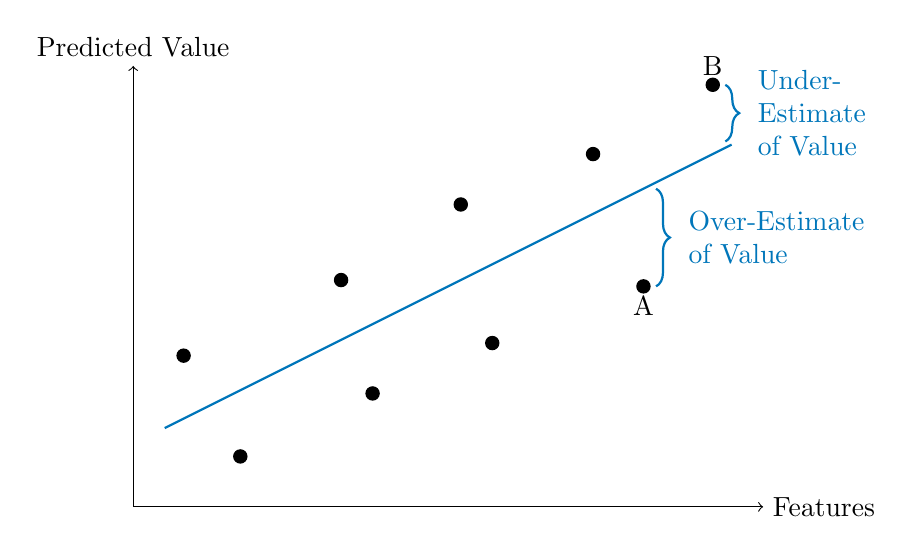
\begin{tikzpicture}[scale=0.8]
        % Axes
        \draw[->] (0,0) -- (10,0) node[right] {Features};
        \draw[->] (0,0) -- (0,7) node[above] {Predicted Value};

        % Regression line: y = 0.5x + 1
        \draw[thick, blue] (0.5, 1.25) -- (9.5, 5.75);

        % 9 points scattered around the line
        \filldraw (0.8, 2.4) circle (3pt);
        \filldraw (1.7, 0.8) circle (3pt);
        \filldraw (3.3, 3.6) circle (3pt);
        \filldraw (3.8, 1.8) circle (3pt);
        \filldraw (5.2, 4.8) circle (3pt);
        \filldraw (5.7, 2.6) circle (3pt);
        \filldraw (7.3, 5.6) circle (3pt);
        \filldraw (8.1, 3.5) circle (3pt) node[below] {A};
        \filldraw (9.2, 6.7) circle (3pt) node[above] {B};

        % Red brace from point (8.1, 3.5) up to regression line (8.1, 5.05)
        \draw[decorate, decoration={brace, amplitude=5pt, mirror}, blue, thick]
            (8.3, 3.5) -- (8.3, 5.05)
            node[midway, right=8pt, blue, align=left] {Over-Estimate\\of Value};

        % Red brace from regression line (9.2, 5.6) up to point (9.2, 6.7)
        \draw[decorate, decoration={brace, amplitude=5pt, mirror}, blue, thick]
            (9.4, 5.8) -- (9.4, 6.7)
            node[midway, right=8pt, blue, align=left] {Under-\\Estimate\\of Value};
    \end{tikzpicture}}
\pause Who will sell if you offer ``Predicted Value''? A? B? Both? Neither?
\end{frame}

\begin{frame}
    \frametitle{}
    \makebox[\textwidth][l]{\hspace{-0.5cm}%
    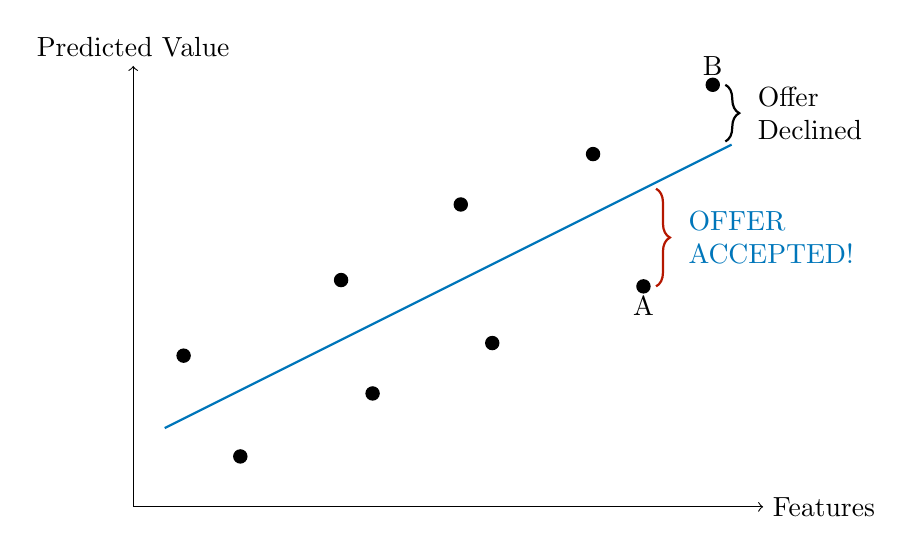
\begin{tikzpicture}[scale=0.8]
        % Axes
        \draw[->] (0,0) -- (10,0) node[right] {Features};
        \draw[->] (0,0) -- (0,7) node[above] {Predicted Value};

        % Regression line: y = 0.5x + 1
        \draw[thick, blue] (0.5, 1.25) -- (9.5, 5.75);

        % 9 points scattered around the line
        \filldraw (0.8, 2.4) circle (3pt);
        \filldraw (1.7, 0.8) circle (3pt);
        \filldraw (3.3, 3.6) circle (3pt);
        \filldraw (3.8, 1.8) circle (3pt);
        \filldraw (5.2, 4.8) circle (3pt);
        \filldraw (5.7, 2.6) circle (3pt);
        \filldraw (7.3, 5.6) circle (3pt);
        \filldraw (8.1, 3.5) circle (3pt) node[below] {A};
        \filldraw (9.2, 6.7) circle (3pt) node[above] {B};

        % Red brace from point (8.1, 3.5) up to regression line (8.1, 5.05)
        \draw[decorate, decoration={brace, amplitude=5pt, mirror}, red, thick]
            (8.3, 3.5) -- (8.3, 5.05)
            node[midway, right=8pt, blue, align=left] {\alert{OFFER} \\ \alert{ACCEPTED!}};

        % Red brace from regression line (9.2, 5.6) up to point (9.2, 6.7)
        \draw[decorate, decoration={brace, amplitude=5pt, mirror}, black, thick]
            (9.4, 5.8) -- (9.4, 6.7)
            node[midway, right=8pt, black, align=left] {Offer\\Declined};
    \end{tikzpicture}}
{\color{red}A will sell}, {\color{blue}B will not}.\\
You lose money!
\end{frame}

\begin{frame}
    \frametitle{}
    \makebox[\textwidth][l]{\hspace{-0.5cm}%
    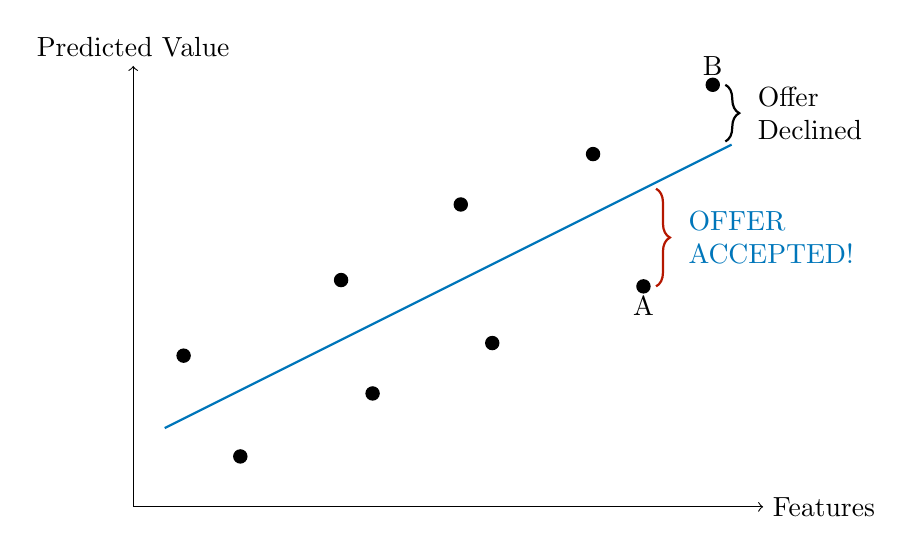
\begin{tikzpicture}[scale=0.8]
        % Axes
        \draw[->] (0,0) -- (10,0) node[right] {Features};
        \draw[->] (0,0) -- (0,7) node[above] {Predicted Value};

        % Regression line: y = 0.5x + 1
        \draw[thick, blue] (0.5, 1.25) -- (9.5, 5.75);

        % 9 points scattered around the line
        \filldraw (0.8, 2.4) circle (3pt);
        \filldraw (1.7, 0.8) circle (3pt);
        \filldraw (3.3, 3.6) circle (3pt);
        \filldraw (3.8, 1.8) circle (3pt);
        \filldraw (5.2, 4.8) circle (3pt);
        \filldraw (5.7, 2.6) circle (3pt);
        \filldraw (7.3, 5.6) circle (3pt);
        \filldraw (8.1, 3.5) circle (3pt) node[below] {A};
        \filldraw (9.2, 6.7) circle (3pt) node[above] {B};

        % Red brace from point (8.1, 3.5) up to regression line (8.1, 5.05)
        \draw[decorate, decoration={brace, amplitude=5pt, mirror}, red, thick]
            (8.3, 3.5) -- (8.3, 5.05)
            node[midway, right=8pt, blue, align=left] {\alert{OFFER} \\ \alert{ACCEPTED!}};

        % Red brace from regression line (9.2, 5.6) up to point (9.2, 6.7)
        \draw[decorate, decoration={brace, amplitude=5pt, mirror}, black, thick]
            (9.4, 5.8) -- (9.4, 6.7)
            node[midway, right=8pt, black, align=left] {Offer\\Declined};
    \end{tikzpicture}}
What happened?\\
\pause Did you lose money because your model was bad?
\end{frame}


\end{document}